\chapter{Background}
\label{ch:Chapter2}

This chapter provides background that is required for understanding the mechanisms of our technique. We provide a short summary of conventional control theory systems followed by DNN based systems, and the different roles of people in the work. We finally end the chapter with a formal definition of our problem statement. 



%We consider a closed-loop system as shown in Figure 2, with sensors as the inputs to the DNN and the actuators that take the output from the DNN based controllers. We describe the model for CPS, followed by the DNN controller model, attack model formalism and the problem statement.

%\aarti{Should the diagram be more descriptive with DNNs in the middle?}
\iffalse
\begin{figure}
	\centering
	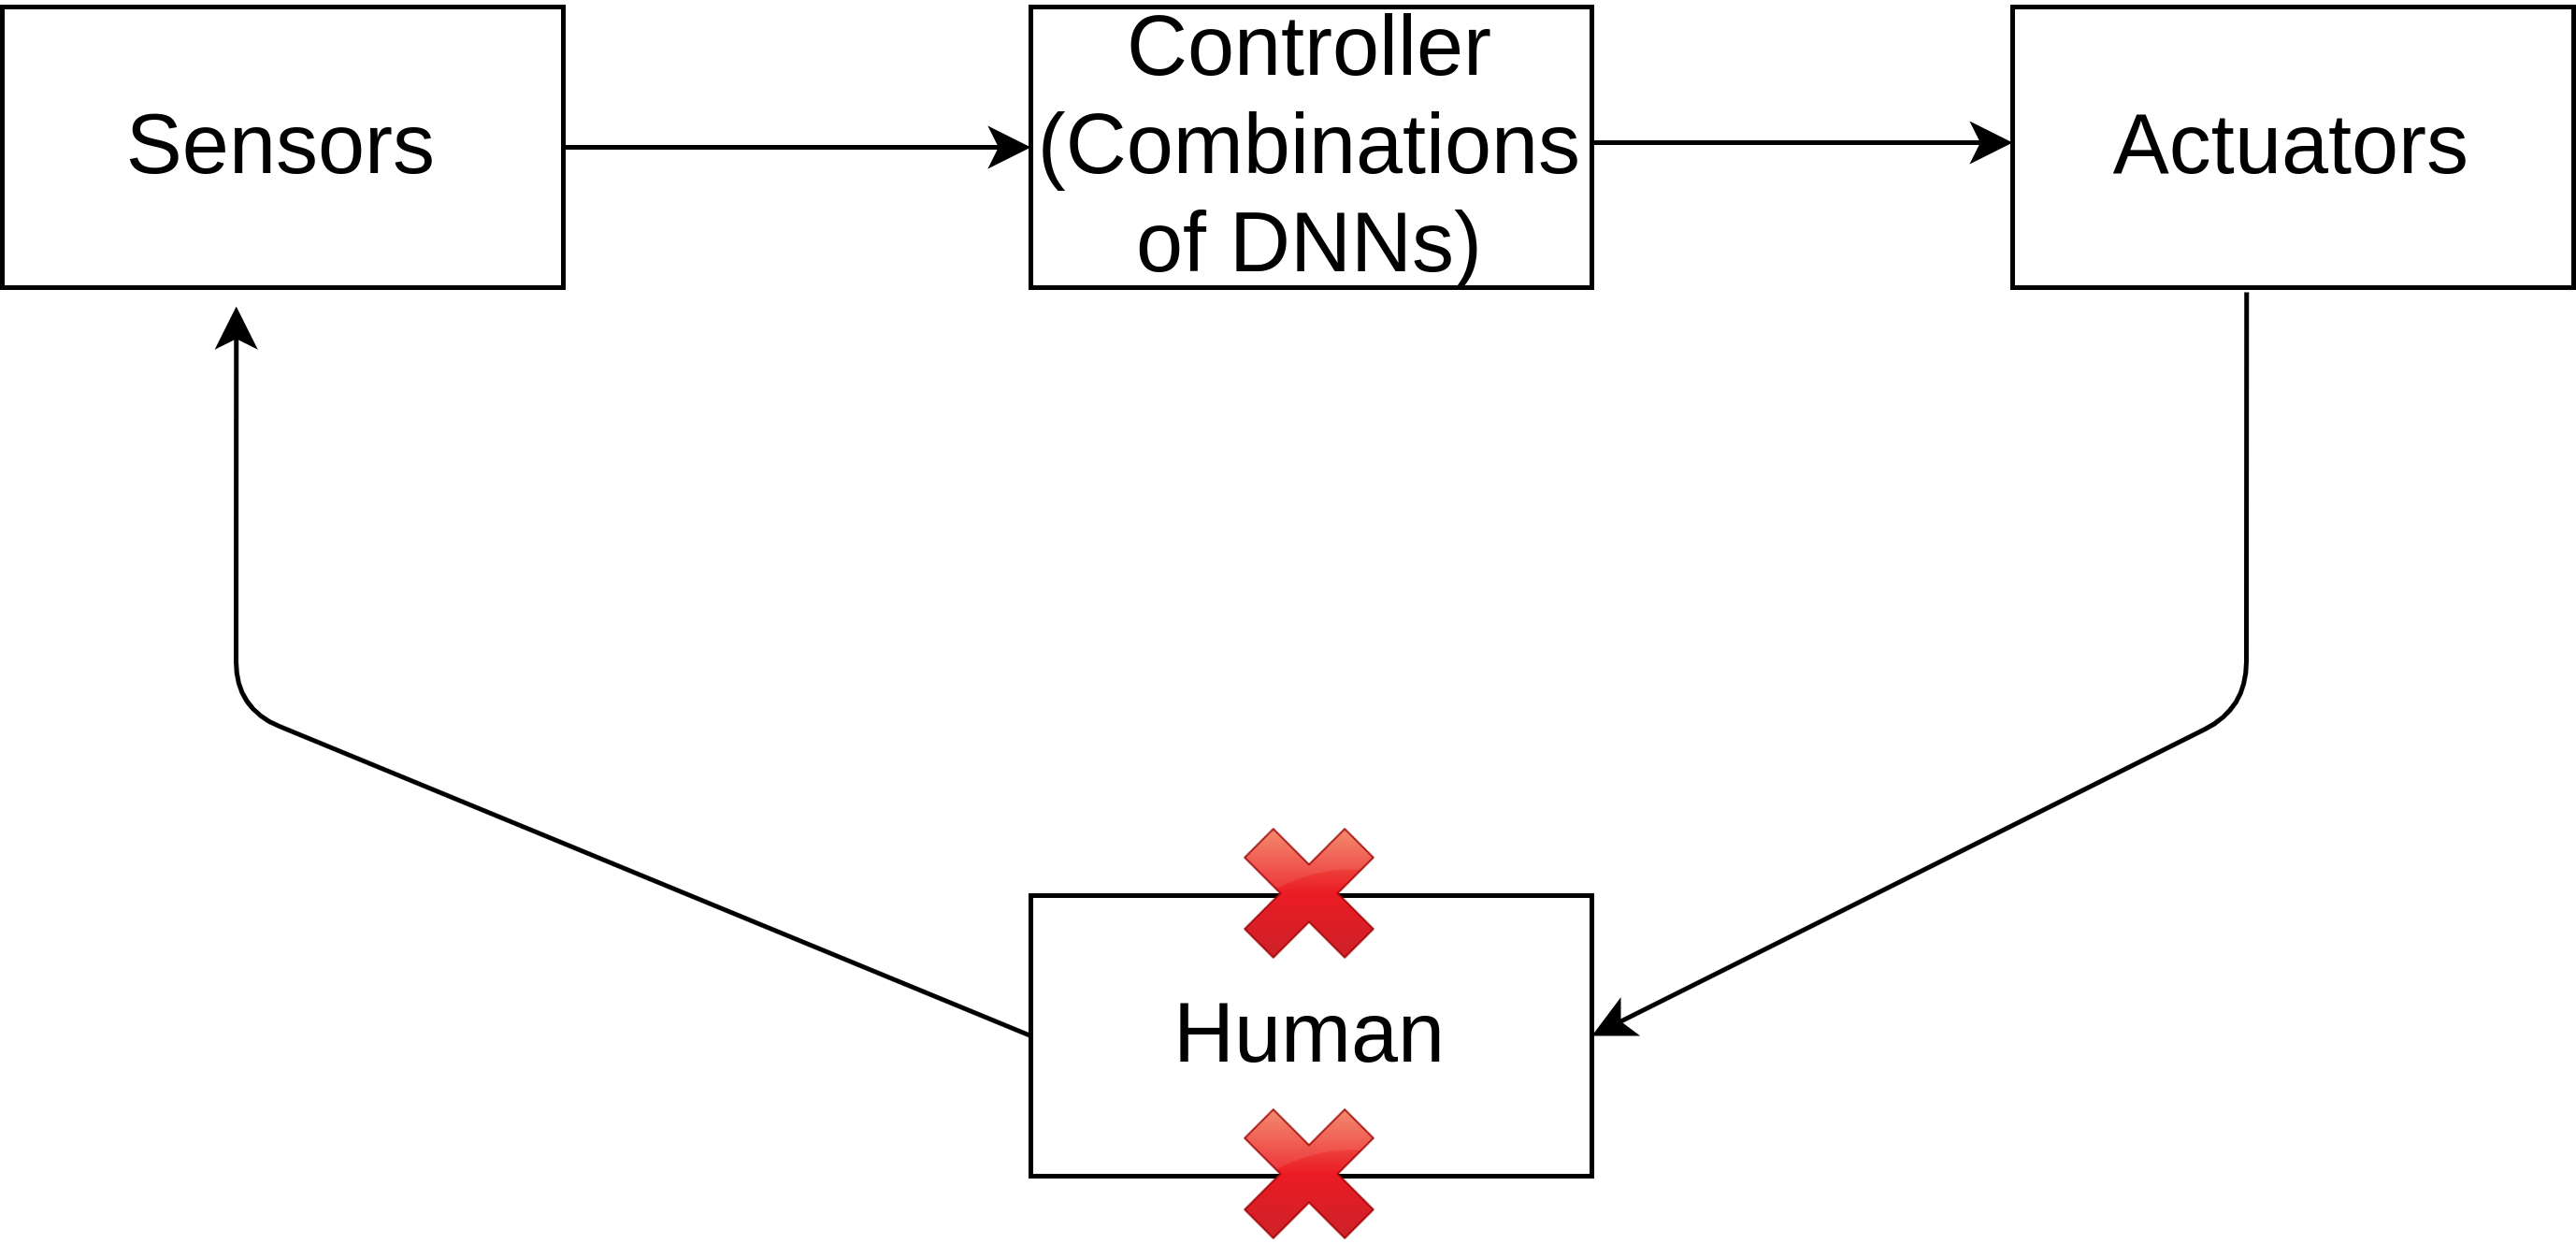
\includegraphics[width=0.7\linewidth]{Images/Systemsdescription}
	\caption[Closed-loop system]{General structure of a closed-loop system without the human involved in the process.}
	\label{fig:systemsdescription}
\end{figure}
\fi

\begin{figure}
	\centering
	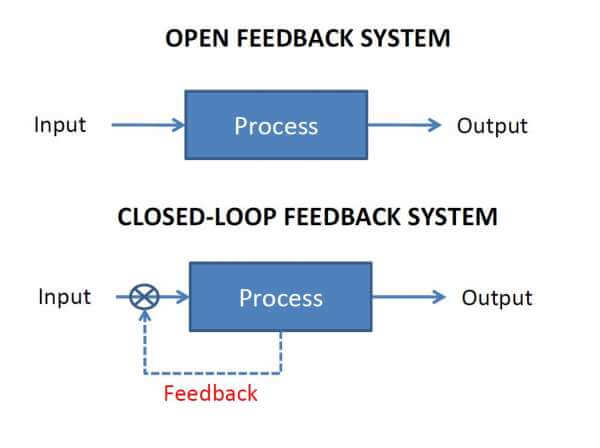
\includegraphics[width=0.7\linewidth]{Images/closedvsopen}
	\caption{General structure of a open and closed-loop systems 
	             Source:https://instrumentationtools.com/open-loop-and-closed-loop-animation/ }
	\label{fig:closedvsopen}
\end{figure}


\section{Cyber-Physical Systems}
\ac{CPS} are systems that combine the cyber part with the physical part that neither could solve alone. CPS based on the data made available make  logical decisions based on the system. For eg. in an insulin pump, the physical data is gathered from the patient which is then used to calculate the  insulin to be injected based on logical formulas and so on the decision making process continues. From Figure 2.1 it can be observed that the decision making process occurs at the controller or the process box where the main logic resides. The data from the physical world is collected from the sensors and the decision making is conducted at the controller and the actuator's job is to physically inject the insulin in the  human which is also the output. 


There are two types of CPS based on the decision making process: open loop and closed loop. In open-loop systems, there is human intervention during the decision making process; as shown in Figure 2.1 the human is a part of the loop where the human keeps a track of the decisions being taken by the controller. 	In closed-loop systems, there are no regular human interventions as shown in Figure 2.1. In the latter case understanding different types of security attacks becomes a necessity. In the case of stealthy (or subtle) attacks as described in the attack model section, the closed loop systems are more vulnerable hence may not raise alarms. The reason is that the existing error-detection mechanisms are not designed to detect small perturbations from the original inputs under a constrained setting that can cause ripples. In DNN based CPS the decision making is accompanied by other DNNs that keep a track of the upper and the lower bounds for error-detection. 

\section{Conventional Controllers for CPS}

%How does a controller work in a conventional setting
A conventional controller takes in the inputs collected through the sensors and processes the input for mode (or state) estimation. There are multiple modes  modeled inside the controller for different scenarios. For eg. in a quadcopter, there are modes for windy flights or normal flights. These modes are important because during a windy weather the flight will have to ensure that the drone is stable and will have to be represented differently as compared to a normal wind flight. Based on the inputs or data collected from the sensors modes are selected. Every mode consists of a different set of equations because every mode represents a different scenario. The outputs are calculated based on the mode that then calculates the next action to be taken by the system. Figure 2.2 shows a position control system of a quadcopter \cite{inbook}. The input values use the derived version of the equations that are used in decision making. 

\begin{figure}
	\centering
	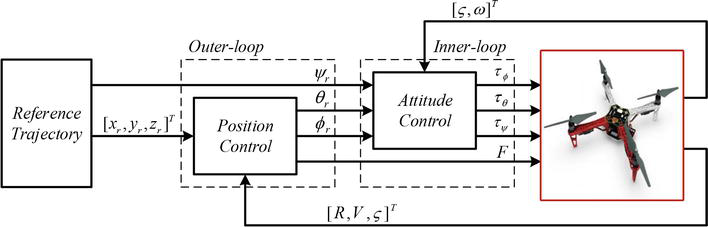
\includegraphics[width=0.7\linewidth]{Images/controltheory}
	\caption{The block diagram of the position control system of the quadcopter.
	}
	\label{fig:controltheory}
\end{figure}


%How are they modeled
These modes are modeled using classical control theory that is represented as a set of equations. These equations are designed by domain experts. For example the model for a medical system such as \ac{APS} can be designed only if the specifications are known for the medical system. A part of the specifications such as the important parameters (insulin, blood glucose etc. in APS) and their threshold values are be provided by domain (in this case medical) experts. Another important aspect for designing control systems is the  modeling precise relations between the parameters. This is possible in systems such as APS because it is a small systems. However, designing the precise mathematical relations for systems such as self-driving cars can be tedious. Therefore, \ac{DNN} have played a huge role in moving the field of autonomous vehicles forward by building models through data. 

  



\section{DNN Based Controller}
The classical controller model is being replaced by DNN based controllers for CPS as shown in  Figure 2.3. The DNN is trained using the data gathered from the traditional control equations. However, during real-time analysis the DNN control is shown to take expert decisions in case of undefined cases. As shown in Figure 2.3 the DNN is the controller and during the training phase the weights and the bias are decided which allows it to control the trajectory in real time. 

One example is the DNN based controller designed by Dutta et al. \cite{Dutta_Others__2018__Robust}. Dutta et al. model robust DNN using available patient data to predict the output in real-time for an insulin pump. Their controller design is for providing a data-driven approach for an artificial pancreas system (APS) which is also our first system for evaluation. 

\begin{figure}
	\centering
	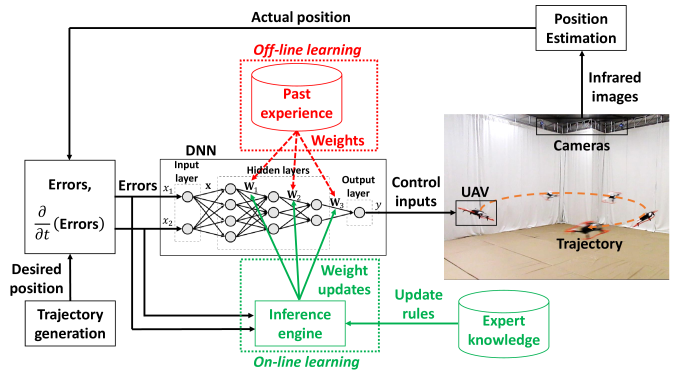
\includegraphics[width=0.7\linewidth]{Images/DNNcontroller}
	\caption{Illustration of how DNN controllers are replacing conventional controllers. The DNN is trained offline using input-output data obtained from different trajectories from a conventional controller. The DNN is shown to perform better than a conventional controller during real-time analysis for decision making.}
	\label{fig:dnncontroller}
\end{figure}

\begin{figure}
	\centering
	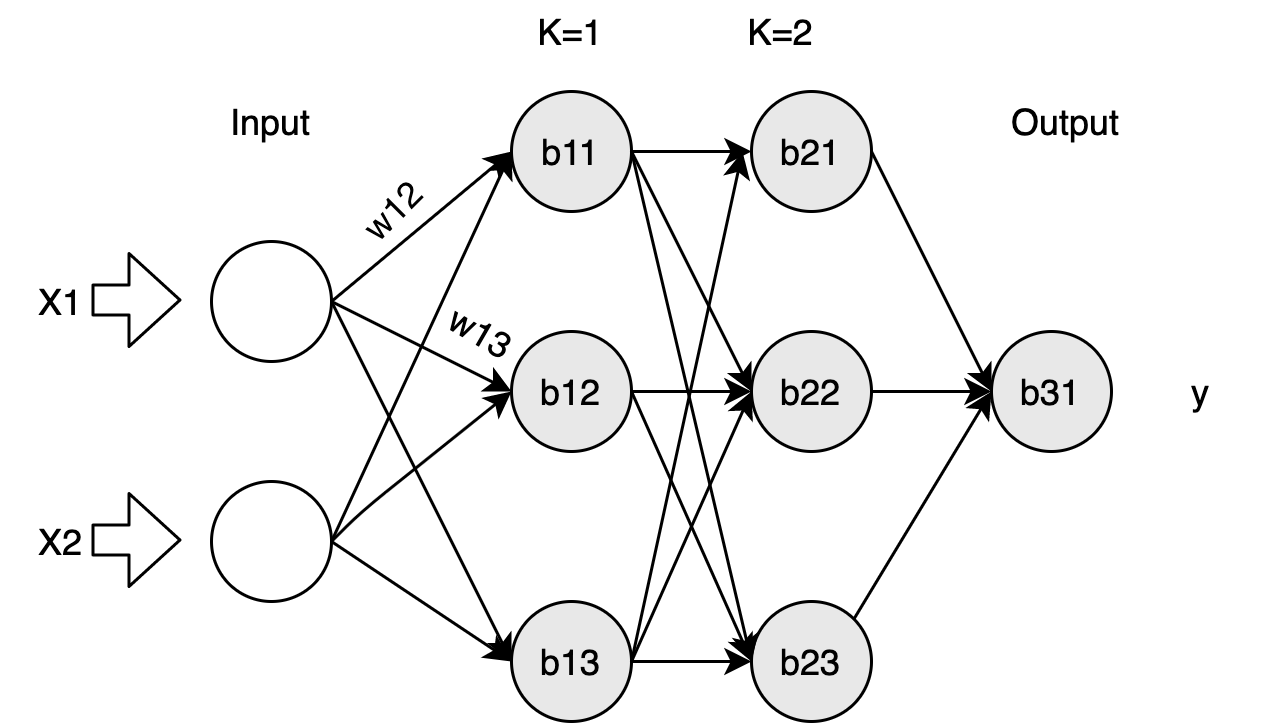
\includegraphics[width=0.7\linewidth]{Images/DNNstructure}
	\caption[DNN structure]{DNN controller structure with two hidden layers K=1,2, two inputs x1 and x2 and one output y. This is an example of a fully connected network.}
	\label{fig:dnn-controller}
\end{figure}

%Intro to the DNN structure
To explain the DNN model in a simple way, we consider a feed-forward neural network with fully-connected layers. A The feedforward neural network was the first and simplest type of artificial neural network devised \cite{feedforward} In this network, the information moves in only one direction, forward, from the input nodes, through the hidden nodes (if any) and to the output nodes. There are no cycles or loops in the network \cite{Zell}.
 %The attack synthesis technique, however, will scale to other classes of DNNs such as recurrent DNNs or CNNs with some optimizations and modeling changes. 

%What does a DNN controller represent?
%What is a DNN made of?
The DNN controller maps the inputs that are the $x1$ and $x2$ to the output $y$ as per Figure 2.4. A DNN consists of multiple layers in the architecture that allows us to create the input-output mappings. The main components of the DNN are inputs, hidden layers, neurons in each hidden layer, the activation function applied to each layer in the network and the output. \textit{For our purposes to synthesize an attack we consider a trained neural network.} This means that all the components of the DNN are fixed.

%Formal modeling of a DNN for later use when explaining the modeling in MILP
The DNN consists of K layers numbered from 1 to K excluding the input layer.  The input layer can be numbered as K=0 and the final layer or the output is the K$^{th}$ layer.
The architecture can be represented as a function F defined as $F: X \rightarrow Y$ where the inputs X are mapped to the output Y and are composed of multiple layers. 

\begin{align*}
F(x) &= F_K \circ F_{K-1} \circ F_{K-2} ....... \circ F_1(x),    (1) \\
or \\
F(x) &= F_K ( F_{K-1}( F_{K-2} .......  (F_1(x)))),    (1) \\
\end{align*} 

$F_K$ represents the K$^{th}$ layer of the network. Each layer K$_{i}$, 
$i$ $\epsilon$ \{1,.,.,.,.,K\} consists of the smallest elements of a DNN called neurons as demonstrated in Figure 2.4.  Each neuron has a bias associated with it. Every neuron from the previous layer is connected to every neuron in the next layer. This is the property of a fully-connected network. 

Each output layer computes its output through the following formula. 
%\aarti{Check the consistency of symbols one more time. }

\begin{align*}
F_i(x) &= \upsigma(W_iX + b_i) ,  i = 1,.....,K, (2)  \\
\end{align*}

$\upsigma$ is the abstraction for different activation functions that can be used to model the DNN. There are multiple types of activation functions which all come with different modeling capabilities such as ReLU ($f(x) = max {0,x}$) as shown in Figure 2.3, logistic $f(x)=1/(1+ exp(-e))$
 Our tool focuses on using Rectified Linear Unit (ReLU) as shown in Figure 2.3 since it is empirically seems to work well and converged much more quickly than a Sigmoid  activation function as shown by Krizhevsky et al. in \cite{10.1145/3065386}.  %It is also piecewise linear so we can model it using MILP encoding. 

\begin{align*}
F_i(x) &= ReLU(W_ix + b_i) ,  i = 1,.....,K , (3) \\
\end{align*}


\begin{figure}
	\centering
	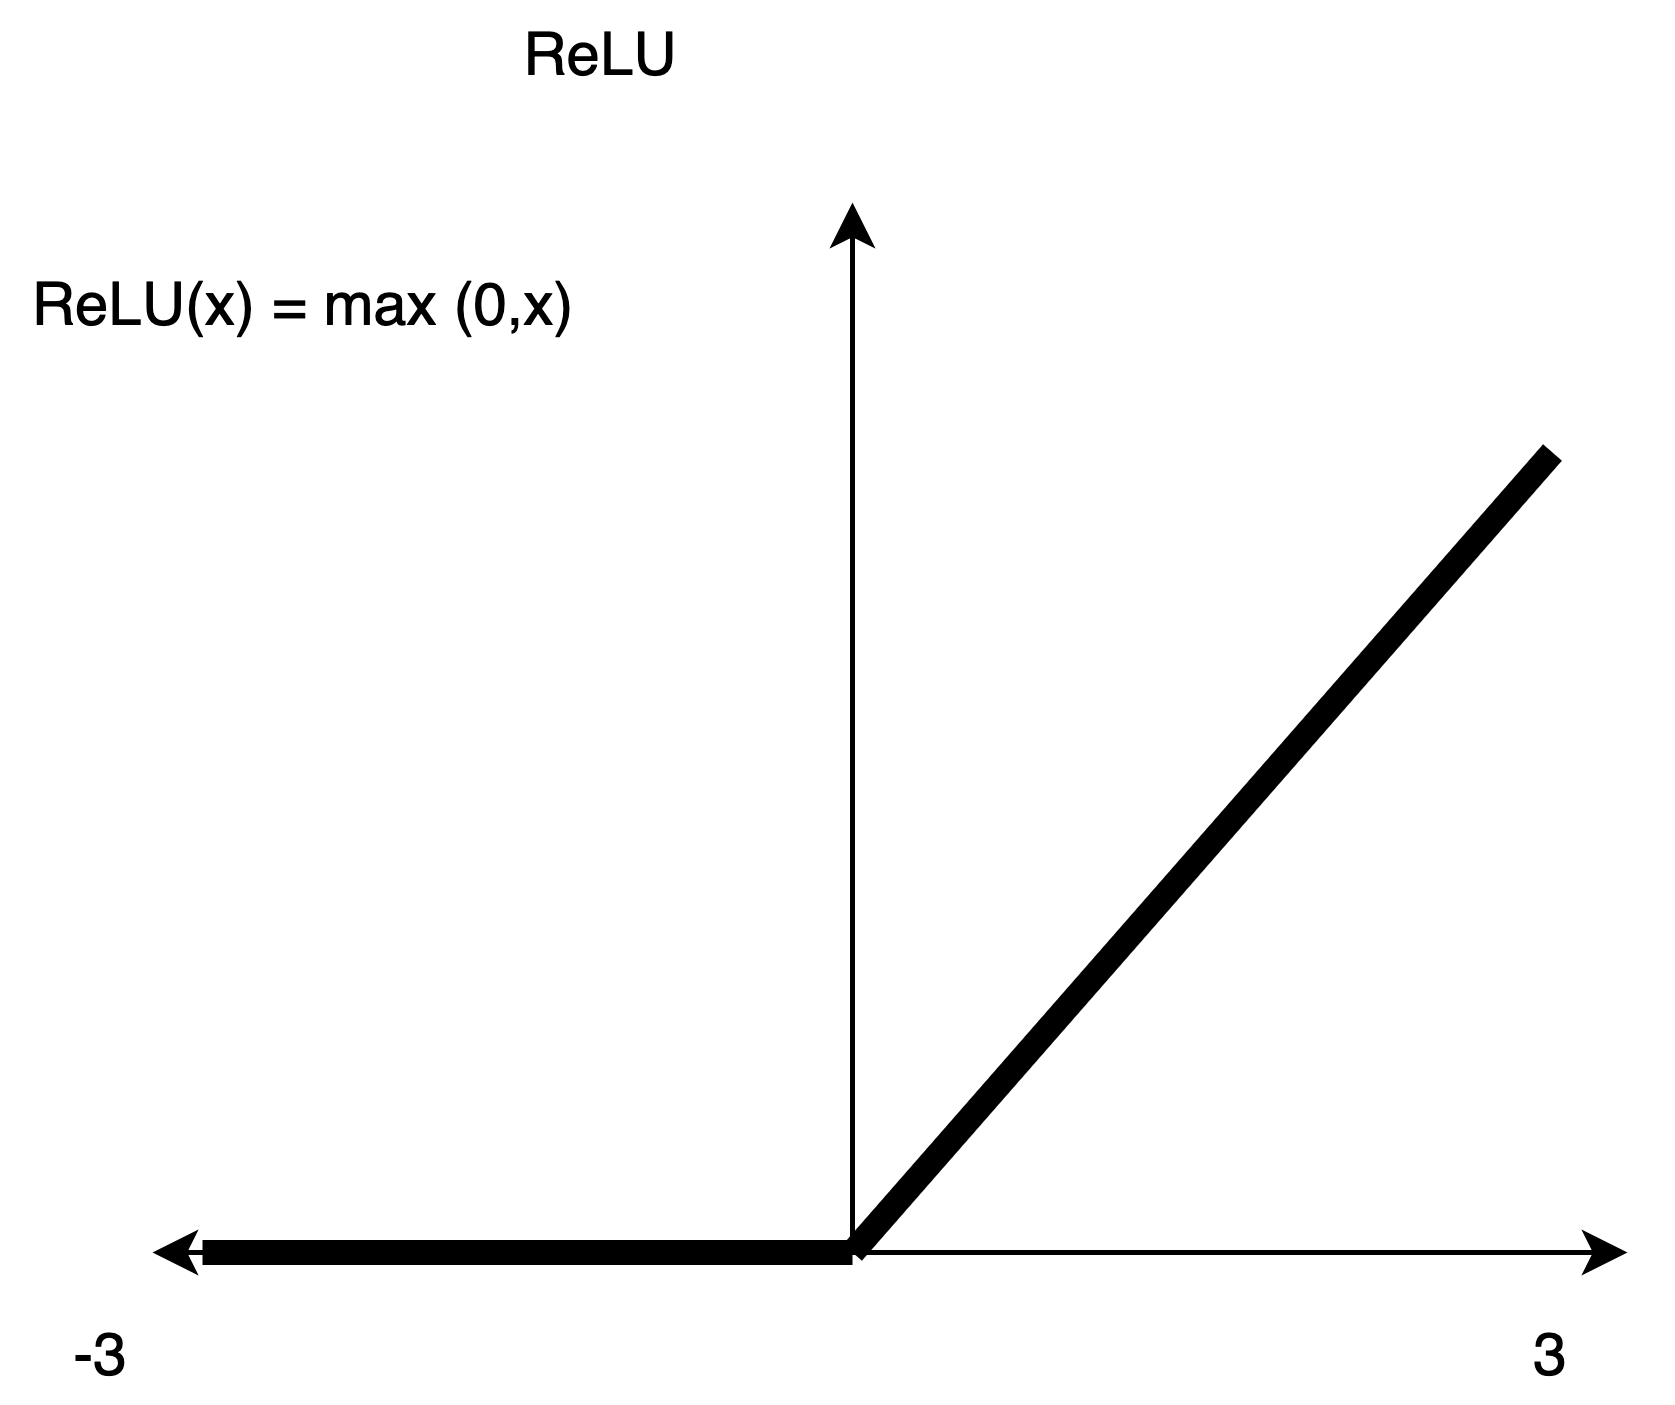
\includegraphics[width=0.7\linewidth]{Images/ReLU}
	\caption[Activation functions]{ReLU activation function}
	\label{fig:ReLU}
\end{figure}
where, for a real vector x, ReLU(x):= max\{0,x\} (per layer).

%During the training of the network, the parameters (weights and bias) are determined; we know those values when we are trying to find attacks on the CPS.

\section{Mapping DNNs to MILP}
The above mentioned formalism allows us to easily map the DNNs to a MILP model. The reason is that the DNN representation can be defined as a set of equations. The notion of non-linearity is introduced in these through the activation functions such as ReLU. The trick here is to define the non-linear activation functions as series of linear functions as shown in Figure 2.6. 

The rest of the equations are directly modeled as a set of constraints for a MILP model and the non-linear activation functions are modeled as a set of linear equations in the MILP model. 

\begin{figure}
	\centering
	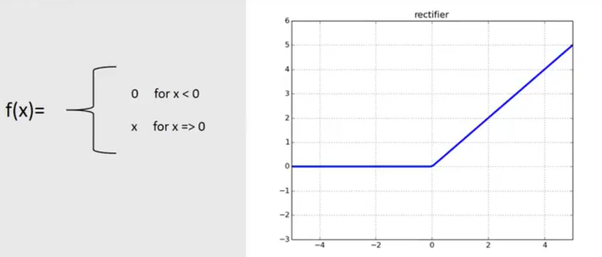
\includegraphics[width=0.7\linewidth]{Images/ReLUbreakdown}
	\caption{ReLU can be broken down into two linear units as shown in the figure for x < 0 and x => 0. This allows us to easily map the DNN equations in MILP models by breaking down the non-linearity inducing function.}
	\label{fig:relubreakdown}
\end{figure}



\section{Roles description}
There are three roles involved in designing and attacking \ac{CPS}.

\begin{enumerate}
	\item \textbf{Specification Designer/Domain Expert:} The domain expert in the realm of \ac{CPS} is responsible for designing the specification documents. For eg. for \ac{APS} the domain expert designs the safe thresholds for the amount of insulin to be injected inside a patient. The domain expert tells values that should trigger alarms in case of a high blood glucose value in a human. 
	
	\item \textbf{System Developer:} These are the people or the designers who based on the specification of the CPS implement the system. For eg. \ac{APS} can be modeled using several different mechanisms. One can use a set of differential equations to design the relations between insulin or blood glucose or one can use \ac{ML} models to build the system models such as decision trees, k-means etc. 
	
	\item \textbf{Attacker:} We are the attackers for the system in the scenario. Our goal is to attack the \ac{CPS} in a stealthy manner. Stealthy here implies we attack the system without getting detected. 
\end{enumerate}



\section{Problem Statement}
%Given that we have the trained DNN model available, in the above section, we identify two problems that we are interested in solving. The first one is identifying the critical inputs in DNN based CPS and the second is synthesizing \attack with minimal cost. 

Given we have a trained DNN with fixed parameters our goal is to understand if the well-known FDI attacks in classical control theory are also valid in the DNN based CPS.
\begin{problem}
	How can we identify the critical inputs in a DNN?
\end{problem}

%Problem 2 is a follow up to the first problem. 

\begin{problem}
	What is the smallest perturbation to the critical input(s) that can result in ripple attacks in a limited time?
\end{problem}
%\smi{\attack is no longer in italics here, do we want to fix this? - interesting}

\begin{approach*}
	We abstract the DNN to a MILP problem using the DNN representation as explained above to recognize the critical inputs to synthesize the \attack. We further model \attack specific cost functions to generate the new perturbed inputs for the attacks. 
\end{approach*}
